\documentclass[letterpaper]{article}

\usepackage[mmddyy]{datetime}
\usepackage[margin=1.25in]{geometry}
\usepackage{fancyhdr}
\usepackage{amsmath}
\usepackage{amssymb}
\usepackage{graphicx}

\usepackage{listings}
\usepackage{color}

\definecolor{codeblue}{rgb}{0.2039, 0.5961, 0.8588}
\definecolor{codegreen}{rgb}{ 0.3451, 0.8392, 0.5529}
\definecolor{codedark}{rgb}{  0.2039, 0.2863, 0.3686}
\definecolor{backcolour}{rgb}{0.9176, 0.9255, 0.9333}
\definecolor{codepink}{rgb}{0.9804, 0.5490, 0.7725}

\lstdefinestyle{mystyle}{
    backgroundcolor=\color{backcolour},
    commentstyle=\color{codegreen},
    keywordstyle=\color{codeblue},
    numberstyle=\tiny\color{codedark},
    stringstyle=\color{codepink},
    basicstyle=\footnotesize,
    basicstyle=\footnotesize\fontfamily{\ttdefault}\selectfont,
    breakatwhitespace=false,
    breaklines=true,
    captionpos=b,
    keepspaces=true,
    numbers=left,
    numbersep=5pt,
    showspaces=false,
    showstringspaces=false,
    showtabs=false,
    tabsize=2
}

\lstset{style=mystyle}

\pagestyle{fancy}
\fancyhf{}
\rhead{Cort Breuer}
\chead{\today}
\lhead{ENGRD 2700}
\rfoot{\thepage}

\begin{document}

\begin{lstlisting}[language=R]
     pbinom(46, 100, .5)
\end{lstlisting}

\begin{center}
    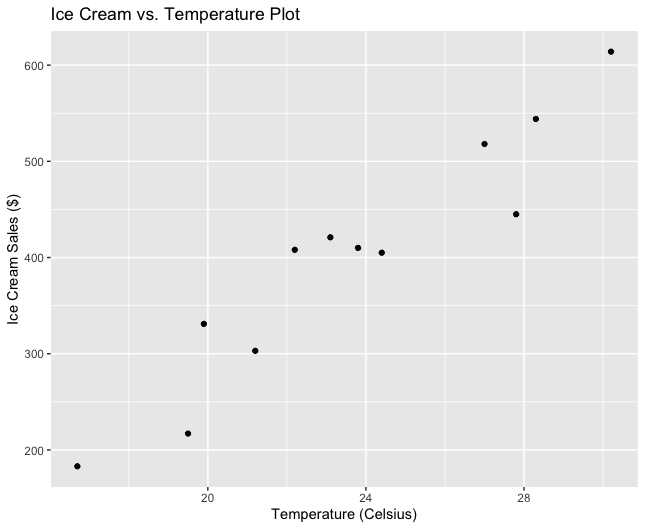
\includegraphics[height=3.5in]{icecream_temp.png}
\end{center}

\vspace*{6pt}

\noindent \textbf{\huge{Problem Set 7}}

\bigskip

\section*{Question 1}

100 service times with a sample mean of 9 minutes and standard deviation of 6 minutes.

\subsection*{Part A}



\subsection*{Part B}

\newpage

\section*{Question 2}

\subsection*{Part A}

\subsection*{Part B}

\subsection*{Part C}

\newpage

\section*{Question 3}

\subsection*{Part A}

\subsection*{Part B}

\subsection*{Part C}

\newpage

\section*{Question 4}

\subsection*{Part A}

\subsection*{Part B}

\newpage

\section*{Question 5}

Expect that a sub weighs 400g, collect 81 samples and find 95\% confidence interval [393.08, 400.92] for mean sub weight.

\subsection*{Part A}

$$\bar{x} = \frac{393.08 + 400.92}{2} = 397$$

$$CI = \bar{x} + t_{\alpha/2, n-1} \frac{S}{\sqrt{n}}$$

$$400.92 = 397 + 1.96 \frac{S}{\sqrt{81}} \quad \longrightarrow \quad 2 = \frac{S}{9}$$

$$S = 18$$

\subsection*{Part B}

Since $CI \propto n^{-1/2}$, the confidence interval is related to the inverse of the square root of the sample size, so to halve the confidence interval width the sample size would have to be increased to 324.

\subsection*{Part C}

$$\bar{x} = 397 \qquad S = 18 \qquad z(90\%) = z(.05) = 1.645 \qquad z(99\%) = z(.005) = 2.576$$

$$CI = \Big[ \bar{x} - z \frac{S}{\sqrt{n}}, \bar{x} + z \frac{S}{\sqrt{n}}\Big]$$

$$\text{90\% Confidence Interval } = 397 \pm 1.645 \frac{18}{9} = [393.71, 400.29]$$

$$\text{99\% Confidence Interval } = 397 \pm 2.576 \frac{18}{9} = [391.85, 402.15]$$


\end{document}
